\documentclass[UTF8,12pt]{ctexart}
\usepackage{../Writeup}
\title{三维旋转}
\author{Josh-Cena}
\begin{document}
\maketitle
\begin{mdframed}[style=Question]
给定过原点和点$(rx,ry,rz)$的直线$r$,求点$(x,y,z)$绕$r$逆时针旋转$\alpha$(从原点看)后得到的点坐标。
\end{mdframed}

\textbf{前置知识:变换矩阵}

在直角坐标系中,可以把任何一个仿射变换理解为将向量乘以一个变换矩阵——该变换矩阵代表了坐标系的相应变换。举个例子,对于旋转变换:
\begin{figure}[H]
    \centering
    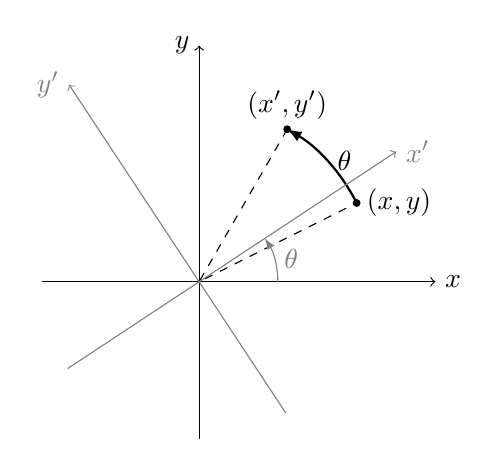
\begin{tikzpicture}[scale=1]
        \draw[->] (-2,0) -- (3,0) node[right] {$x$};
        \draw[->] (0,-2) -- (0,3) node[left] {$y$};
        \draw[-latex,thick] (2,1) node[right] {$(x,y)$} arc ({atan(0.5)}:60:{sqrt(5)}) node[midway,right] {$\theta$} node[above] (a) {$(x',y')$};
        \fill (2,1) circle[radius=0.5mm];
        \fill (a.south) circle[radius=0.5mm];
        \draw[dashed] (a.south) -- (0,0) -- (2,1);
        \draw[-latex,gray] (1,0) arc (0:{60-atan(0.5)}:1) node[midway,right] {$\theta$};
        \draw[->,rotate={60-atan(0.5)},color=gray] (-2,0) -- (3,0) node[right] {$x'$};
        \draw[->,rotate={60-atan(0.5)},color=gray] (0,-2) -- (0,3) node[left] {$y'$};
    \end{tikzpicture}
\end{figure}

我们既可以将其理解为点$(x,y)$旋转到了$(x',y')$,也可以理解成整个坐标系逆时针旋转了$\theta$。旋转后,原本用来定义坐标系的两个正交基
\[\mathbf{x}=\begin{pmatrix}1\\0\end{pmatrix},\mathbf{y}=\begin{pmatrix}0\\1\end{pmatrix}\]
变成了
\[\mathbf{x}'=\begin{pmatrix}\cos\theta\\\sin\theta\end{pmatrix},\mathbf{y}'=\begin{pmatrix}-\sin\theta\\\cos\theta\end{pmatrix}\]

此时,任意一个点$(x,y)$都可以乘上这两个正交基组成的矩阵$\textbf{T}$,得到变换后的坐标。
\[\begin{pmatrix}x'\\y'\end{pmatrix}=\begin{pmatrix}\cos\theta&-\sin\theta\\\sin\theta&\cos\theta\end{pmatrix}\begin{pmatrix}x\\y\end{pmatrix}=\begin{pmatrix}x\cos\theta-y\sin\theta\\x\sin\theta+y\cos\theta\end{pmatrix}\]

三维坐标系需要三个正交基;但方法大致同理。

\textit{题解.} 对于这种旋转问题,我们的通用做法都是先将坐标系变换到一个比较容易处理的位置,再把它转回来。在这题中,我们善于处理的自然是二维的,在$xOy$平面上的旋转:
\begin{figure}[H]
    \centering
    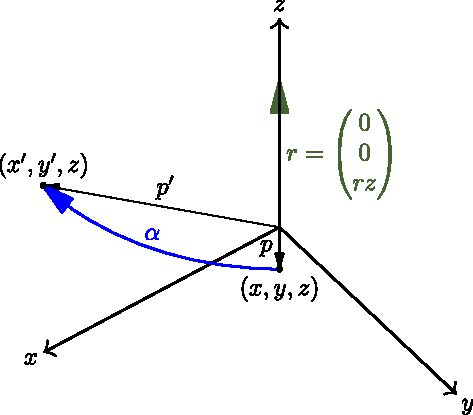
\includegraphics{Rotation1.pdf}
\end{figure}
这个变换是乘以旋转矩阵:
\[p'=\begin{pmatrix}x'\\y'\\z\end{pmatrix}=\begin{pmatrix}\cos\alpha&-\sin\alpha&0\\\sin\alpha&\cos\alpha&0\\0&0&1\end{pmatrix}\begin{pmatrix}x\\y\\z\end{pmatrix}=\begin{pmatrix}x\cos\alpha-y\sin\alpha\\x\sin\alpha+y\cos\alpha\\z\end{pmatrix}\]

那么如何把旋转轴和点转到这个位置?考虑旋转轴的方位角和仰角:
\begin{figure}[H]
    \centering
    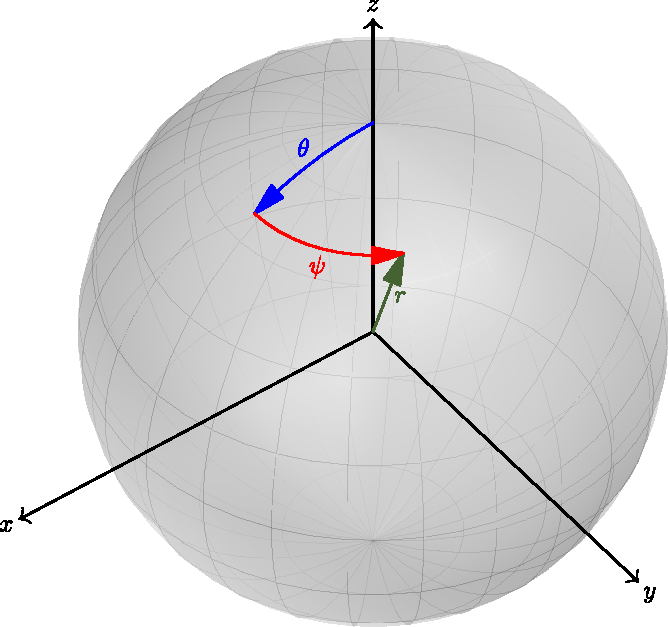
\includegraphics{SphericalSystem.pdf}
\end{figure}
因此只要把$r$绕$z$轴逆时针转$\psi$,再绕$y$轴逆时针转$\theta$即可。叠加两个旋转矩阵:
\begin{equation*}
    \begin{aligned}
        r'&=\begin{pmatrix}\cos\theta&0&-\sin\theta\\0&1&0\\\sin\theta&0&\cos\theta\end{pmatrix}\begin{pmatrix}\cos\psi&-\sin\psi&0\\\sin\psi&\cos\psi&0\\0&0&1\end{pmatrix}\begin{pmatrix}rx\\ry\\rz\end{pmatrix}\\
        &=\begin{pmatrix}x\cos\theta\cos\psi-y\cos\theta\sin\psi-z\sin\theta\\y\cos\psi+x\sin\psi\\x\sin\theta\cos\psi-y\sin\theta\sin\psi+z\cos\theta\end{pmatrix}
    \end{aligned}
\end{equation*}

为了求出$\psi$和$\theta$的值,

\lstinputlisting{./3DRotation.cpp}
\end{document}
